\documentclass{article}
\usepackage[utf8]{inputenc}
\usepackage{graphicx}
\usepackage{float}
\usepackage{hyperref,xcolor}

\title{Kalman Filtering: Case Study 1 \\ (Constant Velocity)}
%\author{Jehangir Amjad }
%\date{August 2016}

\begin{document}

\maketitle

\section{Problem Statement}
Our goal is to track the location (and velocity) of a moving object, e.g. a car, in a 2-dimensional space. The only information available to us is the initial location (and velocity) and a series of noisy measurements of the velocity as the object moves in space. The key assumption of this problem is that the true velocity of the object is known to be a constant. However, the constant velocity is not known to us. 

\section{State Space}
We keep track of the following:

\begin{enumerate}
    \item $x_1$: location in the $x_1$ direction.
    \item $x_2$: location in the $x_2$ direction.
    \item $v_1$: velocity in the $v_1$ direction.
    \item $v_2$: velocity in the $v_2$ direction.
\end{enumerate}

Therefore, let the state vector be represented as:
\[
x &=  \Bigg( \begin{array}{c}
      x_1  \\
      x_2  \\
      v_1  \\
      v_2
 \end{array} \Bigg)
\]

\section{Kalman Equations and Dynamic Model}
\subsection{Kalman Equations}
Reproduced from Wikipedia (below) we have the systems of equations (in matrix format) that need to be solved as part of the Kalman Filtering algorithm. Our challenge is to adapt the problem setting to result in the model that satisfies the form of these equations which will allow us to use Kalman Filtering to track the object's position and velocity.

The Kalman filter model assumes the true state at time k is evolved from the state at (k - 1) according to: \\
\[{\displaystyle \mathbf {x} _{k}=\mathbf {A} _{k}\mathbf {x} _{k-1}+\mathbf {B} _{k}\mathbf {u} _{k}+\mathbf {w} _{k}} 
\] where,

\begin{itemize}
    \item $A_k$ is the state transition model which is applied to the previous state $X _{k-1}$;
    \item $B_k$ is the control-input model which is applied to the control vector $u_k$ (which is not applicable in our setting);
    \item $w_k$ is the process noise which is assumed to be drawn from a zero mean multivariate normal distribution with covariance $Q_k$: \\
    \[
    {\displaystyle \mathbf {w} _{k}\sim {\mathcal {N}}(0,\mathbf {Q} _{k})} 
    \]
\end{itemize}

At time $k$ an observation (or measurement) $z_k$ of the true state $x_k$ is made according to: \\

\[
{\displaystyle \mathbf {z} _{k}=\mathbf {H} _{k}\mathbf {x} _{k}+\mathbf {v} _{k}} \mathbf {z} _{k}
\]
where $H_k$ is the observation model which maps the true state space into the observed space and $v_k$ is the observation noise which is assumed to be zero mean Gaussian white noise with covariance $R_k$.

\[
{\displaystyle \mathbf {v} _{k}\sim {\mathcal {N}}(0,\mathbf {R} _{k})} 
\]
The initial state, and the noise vectors at each step $\{x_0, w_1, …, w_k, v_1 … v_k\}$ are all assumed to be mutually independent.

\subsection{Filtering}
The state of the Kalman filter is represented by two variables: \\

${\displaystyle {\hat {\mathbf {x} }}_{k\mid k}}$, the a posteriori state estimate at time k given observations up to and including at time k; \\

${\displaystyle \mathbf {P} _{k\mid k}}$, the a posteriori error covariance matrix (a measure of the estimated accuracy of the state estimate).

The Kalman filter can be written as a single equation, however it is most often conceptualized as two distinct phases: "Predict" and "Update". The predict phase uses the state estimate from the previous timestep to produce an estimate of the state at the current timestep. This predicted state estimate is also known as the a priori state estimate because, although it is an estimate of the state at the current timestep, it does not include observation information from the current timestep. In the update phase, the current a priori prediction is combined with current observation information to refine the state estimate. This improved estimate is termed the a posteriori state estimate.

Typically, the two phases alternate, with the prediction advancing the state until the next scheduled observation, and the update incorporating the observation. 

\subsubsection{Predict}
\begin{enumerate}
    \item Predicted (a priori) state estimate: {\displaystyle {\hat {\mathbf {x} }}_{k\mid k-1}=\mathbf {A} _{k}{\hat {\mathbf {x} }}_{k-1\mid k-1}+\mathbf {B} _{k}\mathbf {u} _{k}}
    
    \item Predicted (a priori) estimate covariance: {\displaystyle \mathbf {P} _{k\mid k-1}=\mathbf {A} _{k}\mathbf {P} _{k-1\mid k-1}\mathbf {A} _{k}^{\text{T}}+\mathbf {Q} _{k}}
\end{enumerate}

\subsubsection{Update}
\begin{enumerate}
    \item Innovation or measurement residual: {\displaystyle {\tilde {\mathbf {y} }}_{k}=\mathbf {z} _{k}-\mathbf {H} _{k}{\hat {\mathbf {x} }}_{k\mid k-1}} 
    
    \item Innovation (or residual) covariance: {\displaystyle \mathbf {S} _{k}=\mathbf {H} _{k}\mathbf {P} _{k\mid k-1}\mathbf {H} _{k}^{T}+\mathbf {R} _{k}}
    
    \item Optimal Kalman gain: {\displaystyle \mathbf {K} _{k}=\mathbf {P} _{k\mid k-1}\mathbf {H} _{k}^{T}\mathbf {S} _{k}^{-1}} 
    
    \item Updated (a posteriori) state estimate: {\displaystyle {\hat {\mathbf {x} }}_{k\mid k}={\hat {\mathbf {x} }}_{k\mid k-1}+\mathbf {K} _{k}{\tilde {\mathbf {y} }}_{k}} 
    
    \item Updated (a posteriori) estimate covariance: {\displaystyle \mathbf {P} _{k|k}=(I-\mathbf {K} _{k}\mathbf {H} _{k})\mathbf {P} _{k|k-1}}
    
\end{enumerate}


\subsection{Constant Velocity Model}
In our constant velocity model, we have the following:

\subsubsection{Dynamic Matrix, $A_k$}
The Dynamic Matrix, $A_k$, is calculated from the dynamics of motion:

\[
x_{1,k+1} = x_{1,k} + v_{1,k}\cdot \Delta t
\]
\[
x_{2,k+1} = x_{2,k} + v_{2,k}\cdot \Delta t
\]
\[
v_{1,k+1} = v_{1,k}
\]
\[
v_{2,k+1} = v_{2,k}
\]

Hence, 
\[ A_k = \left( \begin{array}{cccc}
1.0 & 0.0 & \Delta t & 0.0 \\
0.0 & 1.0 & 0.0 & \Delta t \\
0.0 & 0.0 & 1.0 & 0.0 \\
0.0 & 0.0 & 0.0 & 1.0 \end{array} \right)
\] 

We define the constant $\Delta t$ later.

\subsubsection{Matrix $B_k$ and vector $u_k$}
In this constant veocity model we have $B_k = 0$ and $u_k = 0$.

\subsubsection{Observation Matrix, $H_k$}
We always observe the velocity, $v_1$ and $v_2$, which results in the following simple model for $H_k$:

\[ H_k = \left( \begin{array}{cccc}
0.0 & 0.0 & 1.0 & 0.0 \\
0.0 & 0.0 & 0.0 & 1.0 \end{array} \right)
\] 

\subsubsection{Measurement Noise Covariance, $R_k$}
We have the following model for measurement noise covariance matrix:

\[ R_k = \left( \begin{array}{cc}
r & 0.0\\
0.0 & r \end{array} \right)
\] 

We define the constant $r$ later. 

\subsubsection{Process Noise Covariance, $Q_k$}
Process noise refers to the modeling of forces that could influence our constant velocity model by creating noise in the form of acceleration disturbance. According to Wikipedia, for this constant velocity model we have:

\[
Q_k = G \cdot G^T \cdot \sigma_v^2
\]

where,

\[ G = \left[ \begin{array}{cccc}
0.5\Delta t^2 & 0.5\Delta t^2 & \Delta t & \Delta t \end{array} \right]
\] 

and we can assume the acceleration process noise $\sigma_v^2 = 8.8 m/s^2$, according to Schubert, R., Adam, C., Obst, M., Mattern, N., Leonhardt, V., & Wanielik, G. (2011). Empirical evaluation of vehicular models for ego motion estimation. 2011 IEEE Intelligent Vehicles Symposium (IV), 534–539.


\section{Initialization}

We initialize the following:

\begin{enumerate}

\item Initial location and velocities, $x_0$.
\[ x_0 = \left( \begin{array}{c}
0.0\\
0.0\\
0.0\\
0.0 \end{array} \right)
\]

\item Time Sampling, $\Delta t = 0.1$
\item Measurement Noise constant, $r = 100.0$
\item Acceleration Process Noise, $\sigma_v^2 = 8.8 m/s^2$

\item Uncertainty matrix, $P_0$.

\[ P_0 = \left( \begin{array}{cccc}
1000.0 & 0.0 & 0.0 & 0.0\\
0.0 & 1000.0 & 0.0 & 0.0\\
0.0 & 0.0 & 1000.0 & 0.0\\
0.0 & 0.0 & 0.0 & 1000.0\\ \end{array} \right)
\]

\end{enumerate}
 

\section{Generating Noisy Measurements}
We can generate the noisy measurements by the following process:

\begin{enumerate}
    \item Let $N = 200$. This is the number of time steps we want to simulate.
    \item Let $v_1 = 20$. This is the true constant velocity.
    \item Let $v_2 = 10$. This is the true constant velocity.
    \item Let $z_1 = v_1 + \mathcal {N}(0,1)$. These are the noisy measurements.
    \item Let $z_2 = v_2 + \mathcal {N}(0,1)$. These are the noisy measurements.
\end{enumerate}
    
The measurements may look like this:

\begin{figure}[H]
  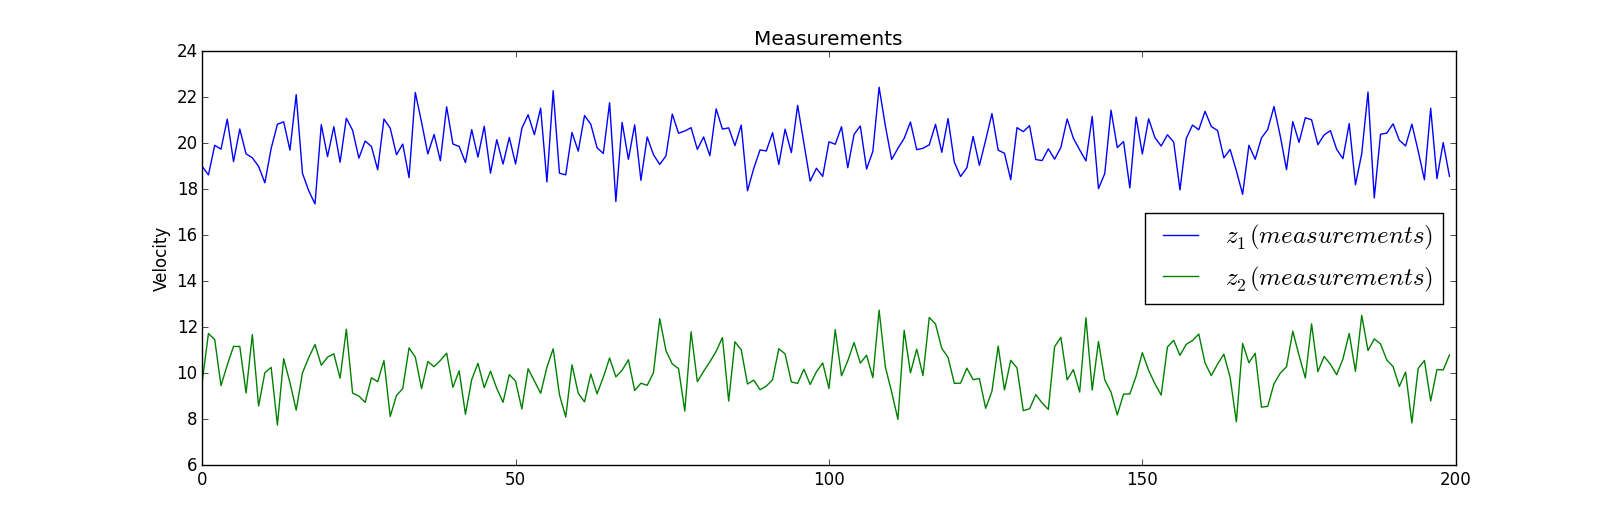
\includegraphics[width=\linewidth]{measurements.png}
  \caption{Noisy measurements of velocity.}
  \label{fig:m1}
\end{figure}

\section{Algorithm}

We now have all the variables defined and noisy measurements ready. Perform the Kalman Filtering steps for $N$ steps, in the following order per iteration:

\begin{enumerate}
    \item Predict steps
    \item Update steps
\end{enumerate}

At each iteration, save all the updated states.

\section{Results}

\subsection{Kalman Gain}

\begin{figure}[H]
  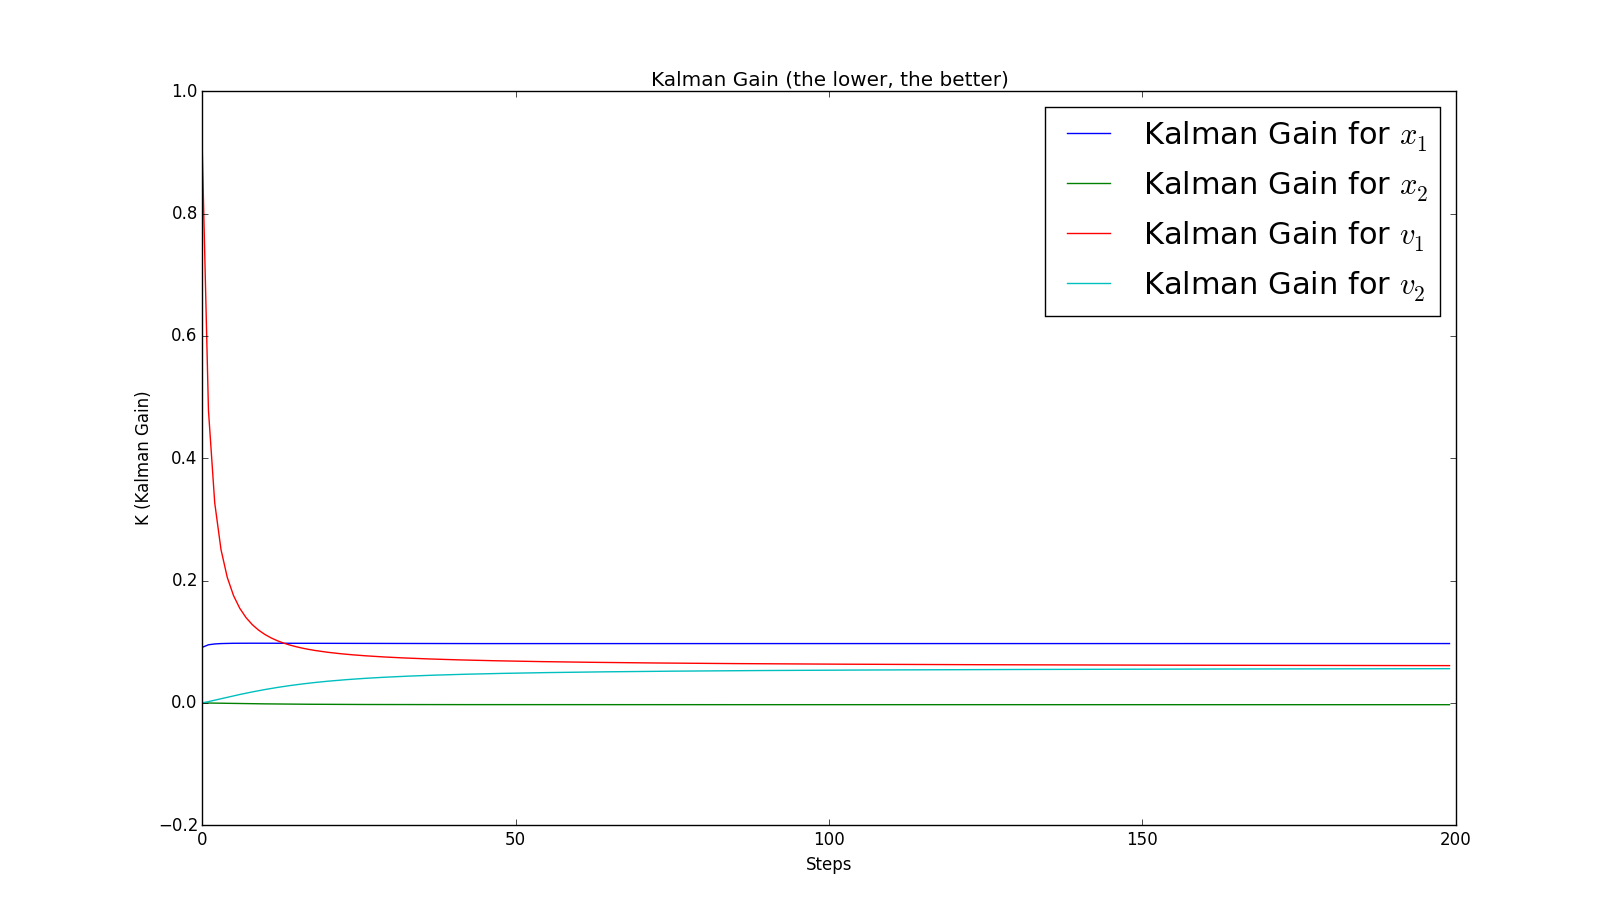
\includegraphics[width=\linewidth]{kalman_gains.png}
  \caption{Kalman Gains, $K_k$ for the position and velocity.}
  \label{fig:m2}
\end{figure}


\subsection{Velocity Tracking}

\begin{figure}[H]
  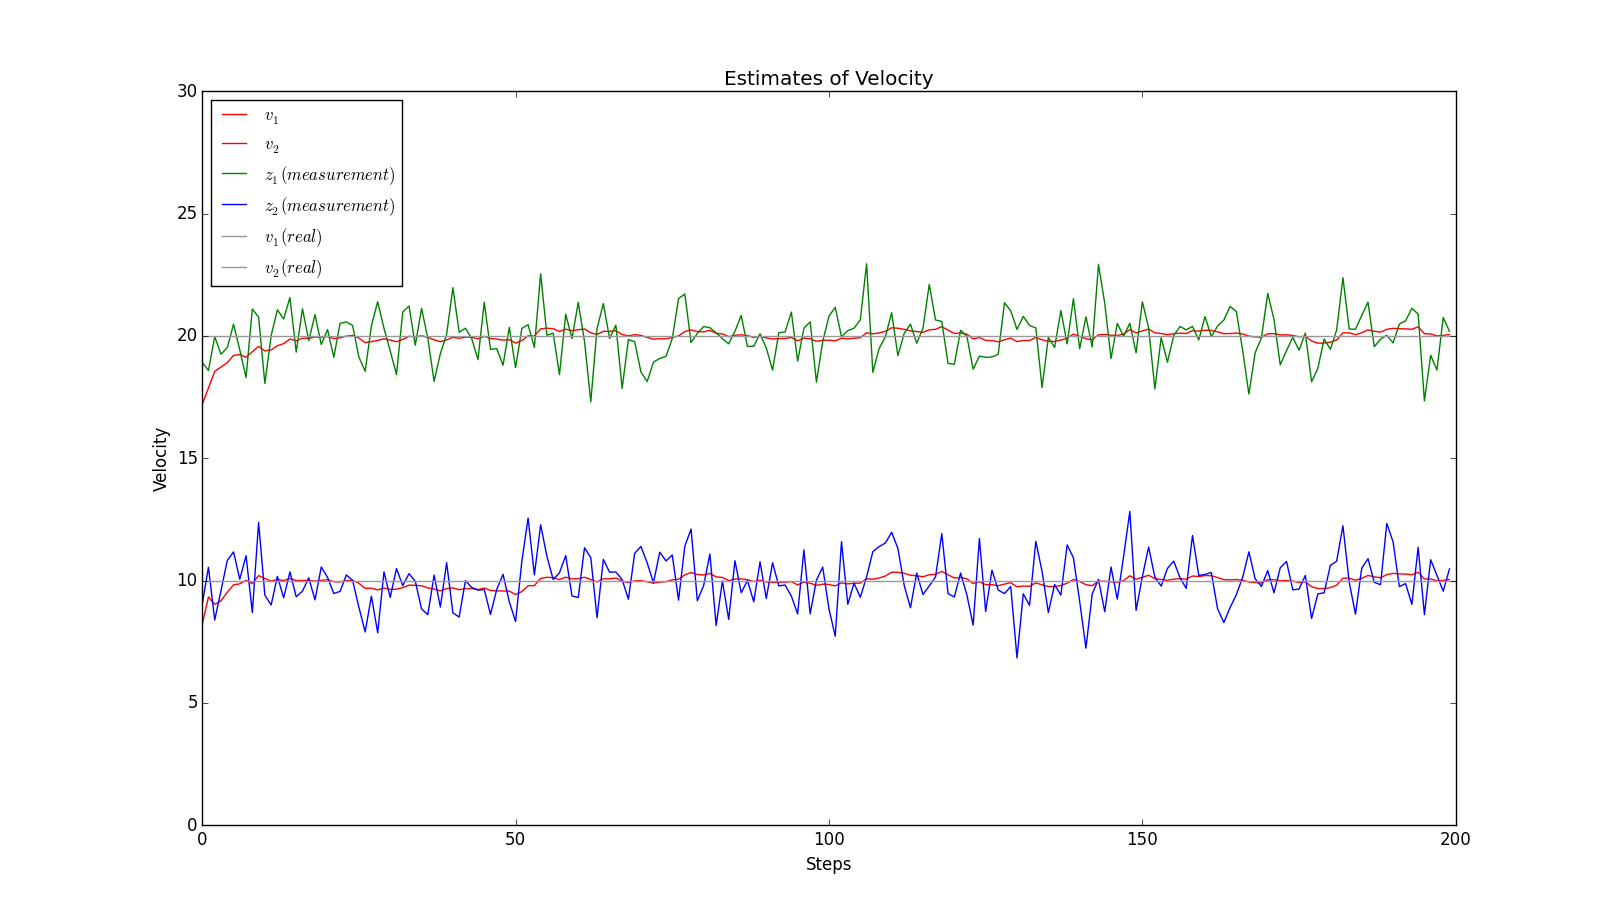
\includegraphics[width=\linewidth]{velocity_states_tracking.png}
  \caption{Velocity estimates (red), noisy velocity estimates (green, blue) and the constant true velocity (gray).}
  \label{fig:m3}
\end{figure}

\subsection{Position Tracking}
Our objective was to track the position of the object. Given the constant velocity assumption, the following shows that the Kalman Filter based estimates do a great job (the resulting path is a straight line on the 2D plot with the expected displacement in each direction).

\begin{figure}[H]
  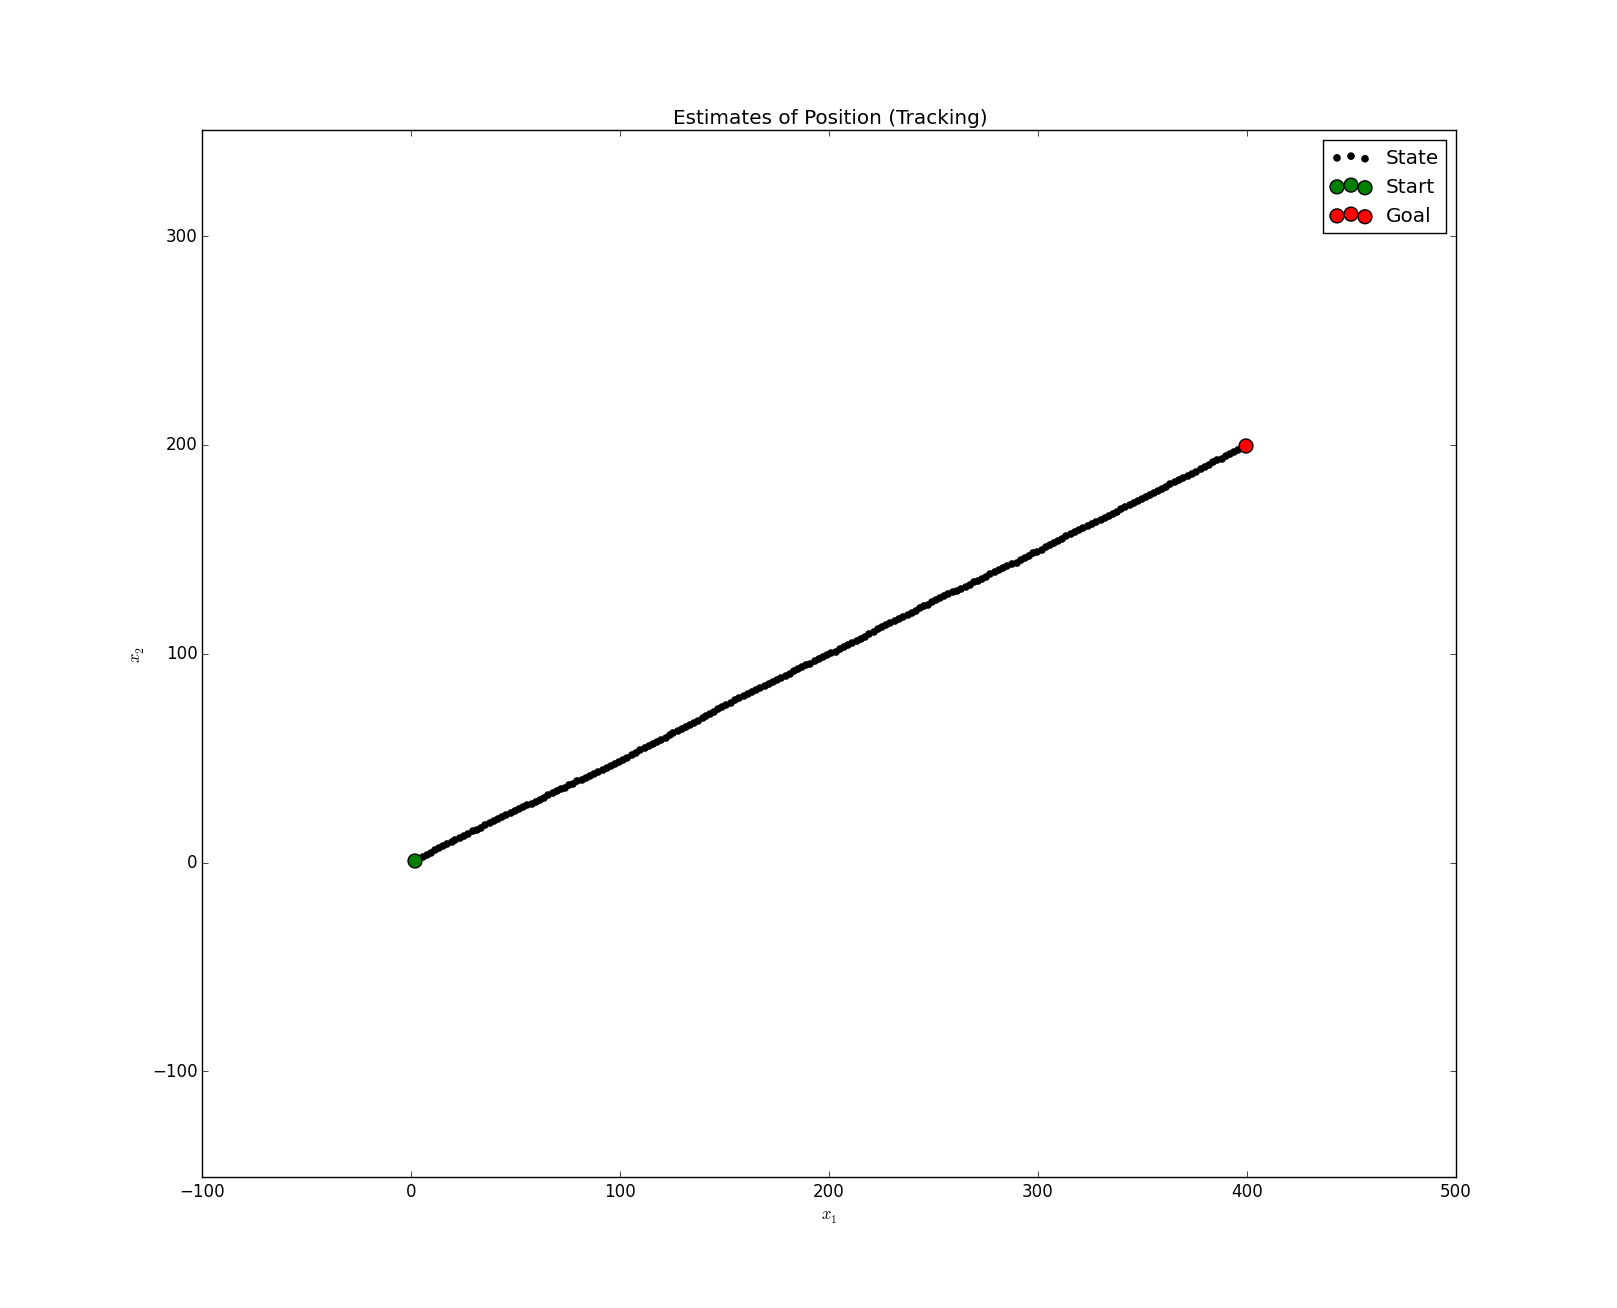
\includegraphics[width=\linewidth]{position_tracking.png}
  \caption{Position estimates in both dimensions, on a 2D plot.}
  \label{fig:m4}
\end{figure}


\section{Greater Measurement Noise}
If the measurement noise was increased, as described below, we see the following effects on the filter.

\begin{enumerate}
    \item Let $z_1 = v_1 + 5 \cdot \mathcal {N}(0,1)$. These are the noisy measurements.
    \item Let $z_2 = v_2 + 5 \cdot \mathcal {N}(0,1)$. These are the noisy measurements.
\end{enumerate}

Notice that the randomness is now 5 orders of magnitude higher resulting in greater noise, as shown below. The tracking is also impacted.

\begin{figure}[H]
  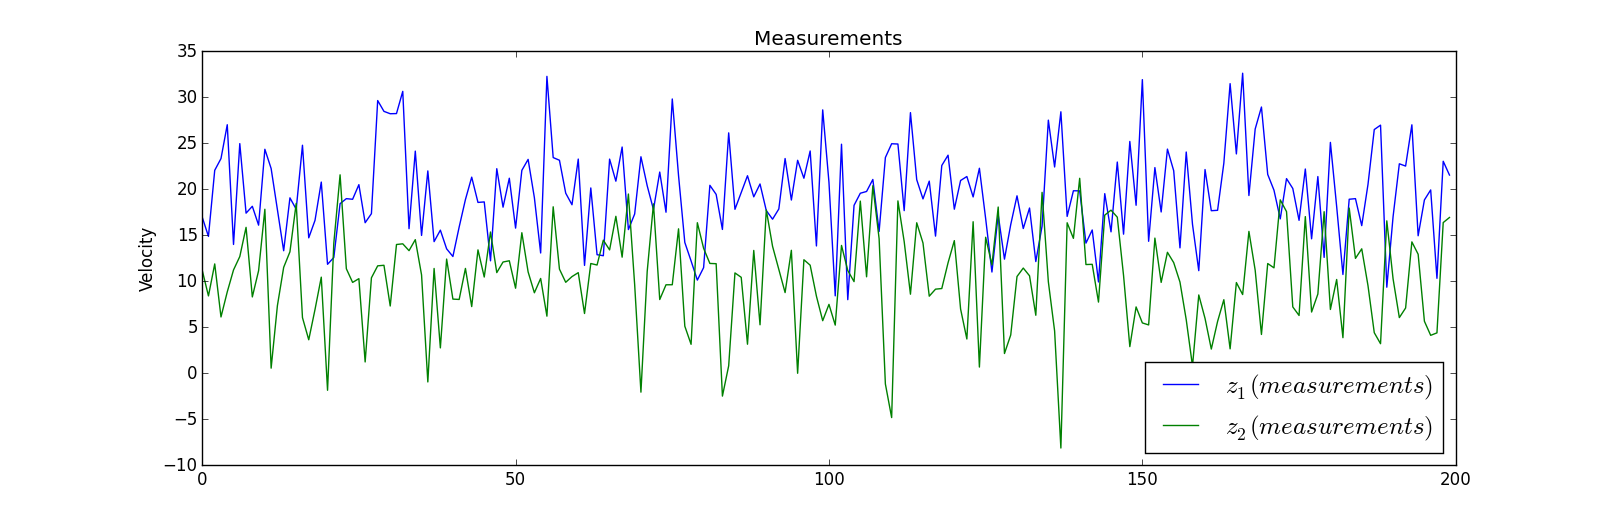
\includegraphics[width=\linewidth]{measurements_greater_noise.png}
  \caption{Greater Noise measurements of velocity.}
  \label{fig:m5}
\end{figure}

\begin{figure}[H]
  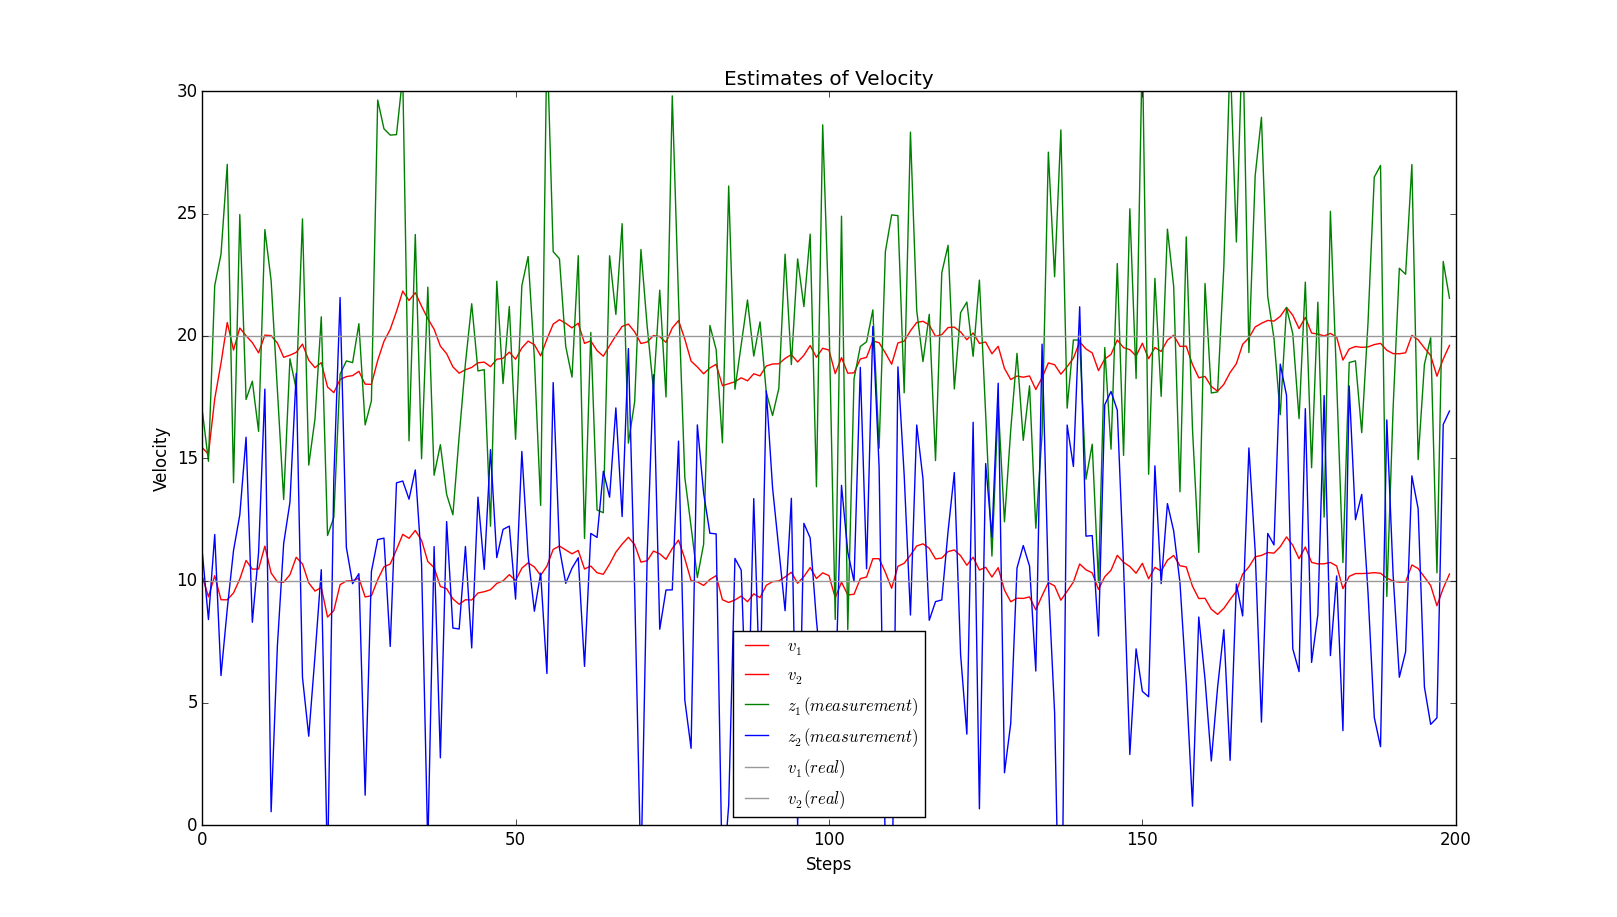
\includegraphics[width=\linewidth]{velocity_states_tracking_greater_noise.png}
  \caption{Velocity estimates (red), noisy velocity estimates (green, blue) and the constant true velocity (gray) with greater measurement noise. Notice how the estimates now follow the noisy measurements more closely.}
  \label{fig:m6}
\end{figure}


\begin{figure}[H]
  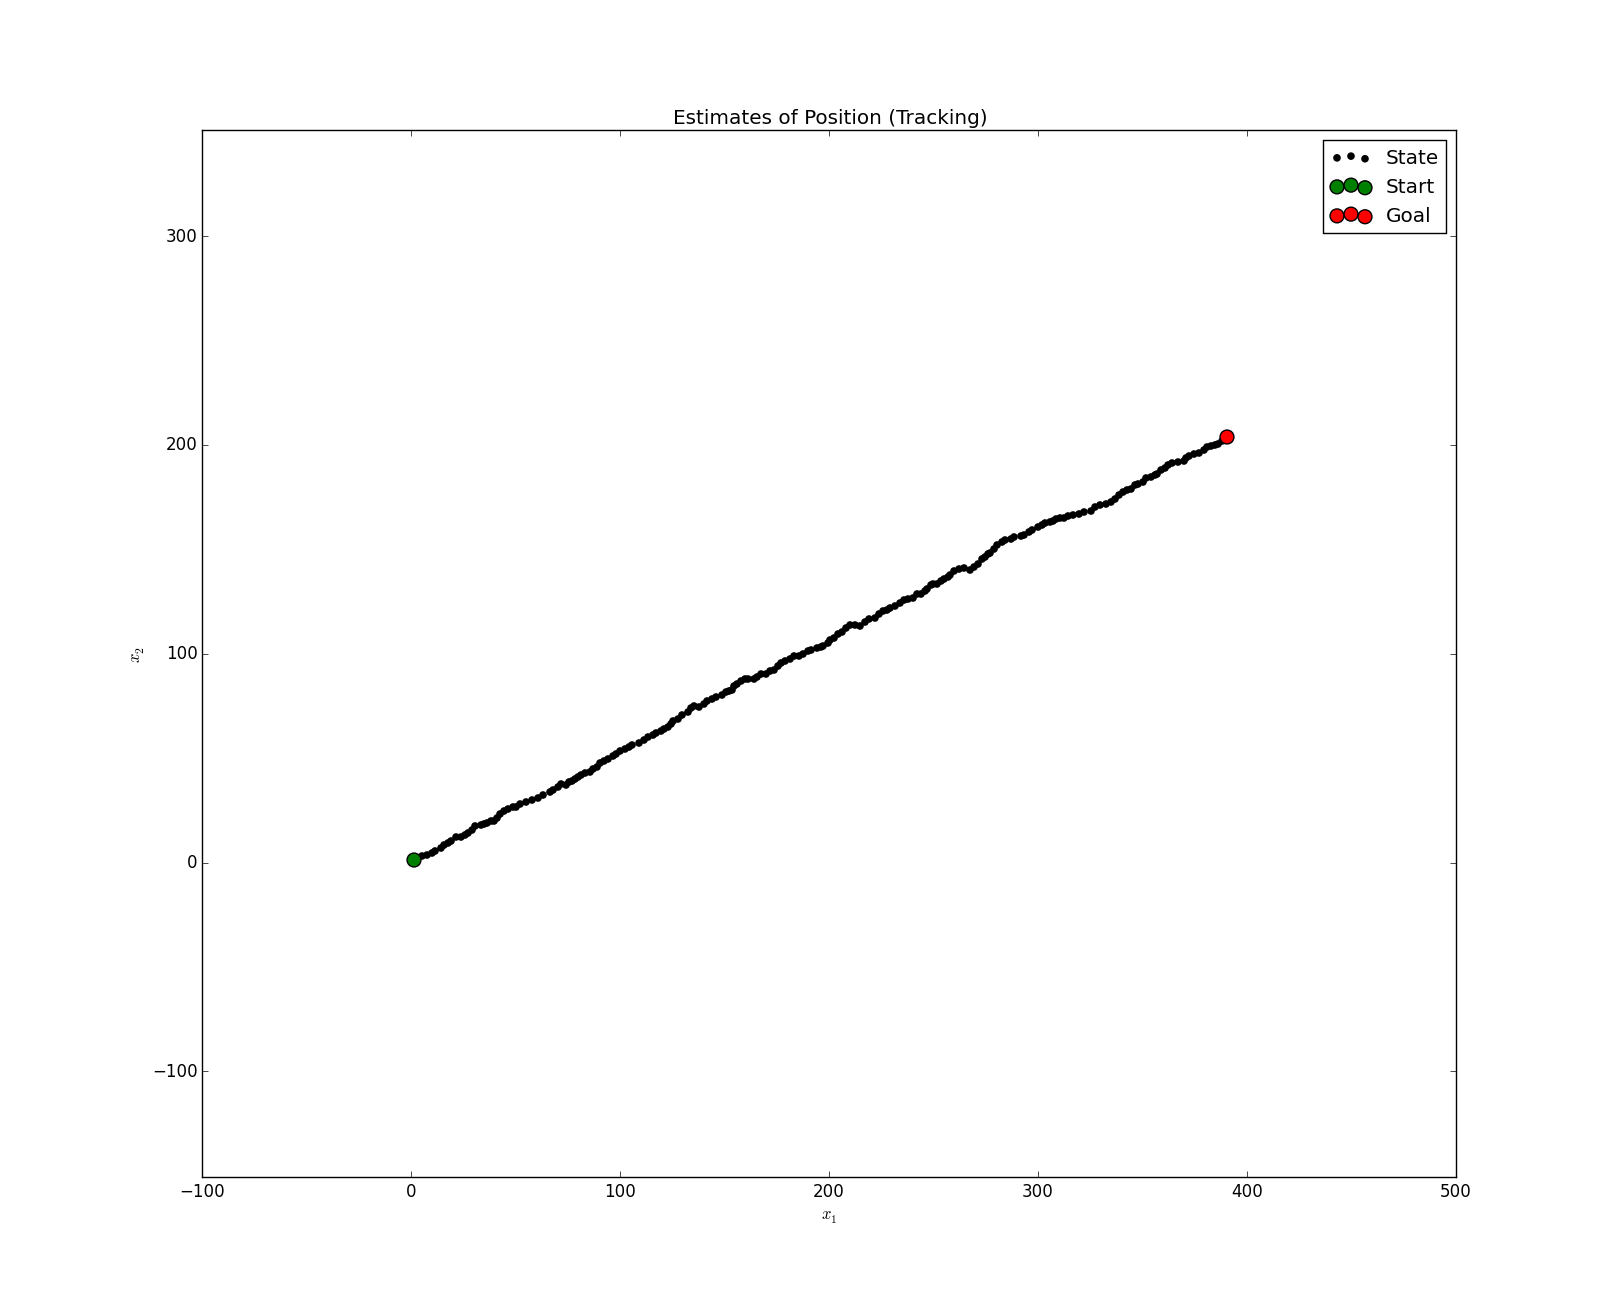
\includegraphics[width=\linewidth]{position_tracking_greater_noise.png}
  \caption{Position estimates in both dimensions, on a 2D plot with greater measurement noise. Notice the line is still roughly straight but with greater variation.}
  \label{fig:m4}
\end{figure}


\section{Source}
Material for this case study was inspired by the following:\\
\url{https://balzer82.github.io/Kalman/} \\

For more details on Kalman Filtering equations used, please check: \\
\url{https://en.wikipedia.org/wiki/Kalman_filter}
\end{document}
